\section{提出的方法}\label{ux63d0ux51faux7684ux65b9ux6cd5}

\section*{Proposed Method}

在多标签眼科疾病识别的域泛化过程中，模型性能主要受到三方面因素影响。首先，同一眼底图像中可能同时存在多种疾病，若模型不能有效建模疾病标签之间以及标签与疾病特征之间的关联，容易产生误检与漏检，从而降低多标签识别性能。其次，源域与目标域之间通常存在分布差异，若模型学习到的特征中包含较多源域特定噪声，则会削弱疾病相关特征的迁移能力，导致域泛化性能下降。此外，隐私保护机制虽然可以降低隐私泄露风险，但也可能通过额外的训练约束影响模型优化过程，因此需要考虑隐私保护与模型性能之间的平衡问题。

In domain generalization for multi-label ocular disease recognition, model performance is mainly affected by three factors. First, multiple diseases may coexist in the same fundus image. If the model cannot effectively capture relevance among disease labels and between labels and disease-related features, false positives and false negatives may occur, degrading multi-label recognition performance. Second, distribution shifts commonly arise between the source domain and target domain. If the learned features contain substantial source-domain-specific noise, the transferability of disease-related features is weakened, resulting in poorer domain generalization performance. In addition, although privacy-preserving mechanisms can reduce privacy leakage risk, they may also affect model optimization through additional training constraints. The balance between privacy preservation and model performance must therefore be considered.

针对上述问题，本文首先将多疾病共存和域偏移不视为两个孤立问题，而是统一到多标签眼科疾病识别的单域泛化框架中进行建模。如\figref{fig:method-framework}所示，所提可解释单域泛化框架主要包括两个部分：Part1.双分支引导域不变特征提取，Part2.自适应标签-特征关联性构建。Part1以 CAM 作为引导，结合双分支 mask 对比学习机制，从单一源域中提取更稳定的域不变特征，缓解源域与未知域之间的分布差异影响。同时CAM能够可视化模型关注区域，增强可解释性；Part2在Part1输出的域不变特征基础上，利用Transformer注意力机制建模标签-标签关联与标签-特征关联性，减少多标签识别中的误检与漏检。两个部分并非独立工作，而是通过特征过滤和注意力一致性约束形成协同：Part1为Part2提供更稳定的域不变特征，Part2进一步约束双分支注意力特征的一致性，从而共同提升域泛化性能。最后，训练过程中集成自适应高斯差分隐私机制，以缓解隐私保护机制对模型性能的影响，并在隐私保护与模型性能之间取得平衡。综合以上，所提方法构建了一个面向多标签眼科疾病识别的可解释与隐私保护单域泛化框架。以下分三小节详细描述各模块的实现细节。

To address these issues, this study does not treat multi-disease co-occurrence and domain shift as separate problems. Instead, they are jointly modeled within a single domain generalization framework for multi-label ocular disease recognition. As shown in \hyperref[fig:method-framework]{Fig.~\ref*{fig:method-framework}}, the proposed interpretable single domain generalization framework consists of two main parts: Part 1, Dual-Branch Guided Domain-Invariant Feature Extraction (DFE), and Part 2, Adaptive Label-Feature Relevance Construction (ARC). Part 1 uses CAM guidance together with a dual-branch mask-based contrastive learning mechanism to extract more stable domain-invariant features from a single source domain, thereby reducing the influence of distribution shift between the source domain and unseen domains. CAM also visualizes model-attended regions and enhances interpretability. Based on the domain-invariant features produced by Part 1, Part 2 uses Transformer attention mechanisms to model label-label relevance and label-feature relevance, reducing false positives and false negatives in multi-label recognition. These two parts are coupled through feature filtering and attention consistency constraints: Part 1 provides more stable domain-invariant features for Part 2, while Part 2 further constrains the consistency of dual-branch attention features, jointly improving domain generalization performance. Finally, an Adaptive Gaussian Differential Privacy mechanism is integrated during training to reduce the impact of privacy preservation on model performance and to balance privacy preservation with model performance. Overall, the proposed method constructs a Privacy-Preserving Interpretable Single Domain Generalization framework for multi-label ocular disease recognition. The implementation details of each module are described in the following three subsections.

\begin{figure}[H]
\centering
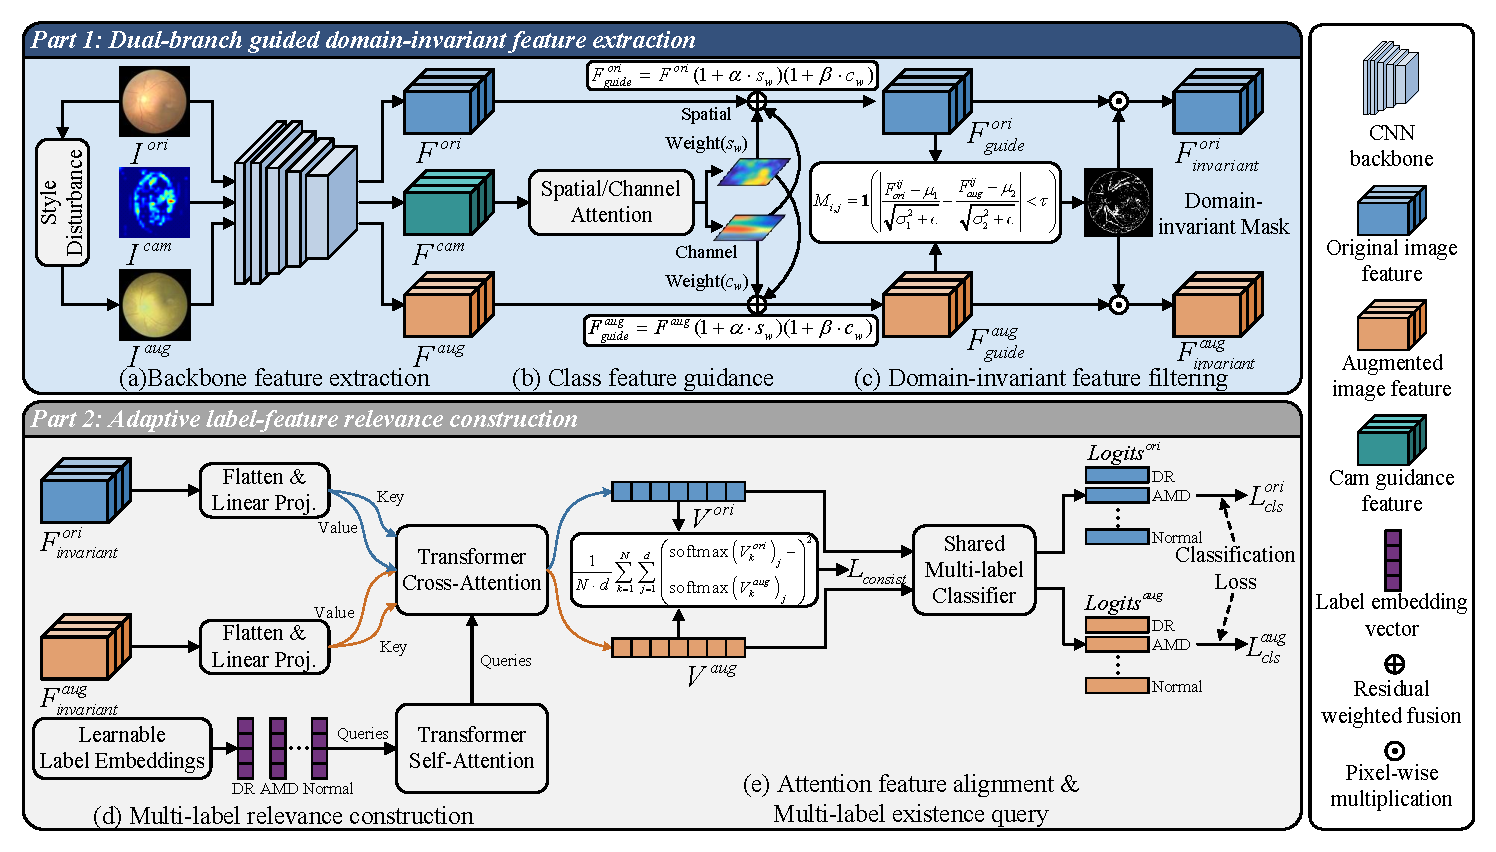
\includegraphics[width=0.96\textwidth]{./images/media/image2_padded.pdf}
\caption{所提可解释单域泛化框架总览。Part1 为双分支引导域不变特征提取（DFE），由 (a)--(c) 组成：首先 (a) 将源域原始图像与源域增强图像输入骨干网络提取双分支特征；同时 (b) 利用 CAM 生成模型关注区域引导，以增强疾病相关区域并抑制背景噪声；最终 (c) 通过双分支 mask 对比学习机制保留两路特征中的高度相似部分，从而提取域不变特征。Part2 为自适应标签-特征关联性构建（ARC），由 (d)--(e) 组成：其中 (d) 利用 Transformer 自注意力机制建模标签-标签关联，再通过交叉注意力机制建立标签-特征关联性，然后由 (e) 利用注意力一致性约束提升注意力特征的稳定性，从而减少多标签识别中的误检与漏检。Part1 和 Part2 协同工作，模型能够在提取域不变特征的同时更有效地建模标签关联，从而共同提升域泛化性能。 Overview of the proposed interpretable single domain generalization framework. Part 1 is Dual-Branch Guided Domain-Invariant Feature Extraction (DFE), consisting of (a)--(c): (a) original source-domain images and augmented source-domain images are first fed into the backbone to extract dual-branch features; (b) CAM is used to generate model-attended region guidance, which enhances disease-related regions and suppresses background noise; and (c) a dual-branch mask-based contrastive learning mechanism retains highly similar components between the two feature branches to extract domain-invariant features. Part 2 is Adaptive Label-Feature Relevance Construction (ARC), consisting of (d)--(e): (d) Transformer self-attention is used to model label-label relevance, and cross-attention is then used to establish label-feature relevance; (e) attention consistency constraints improve the stability of attention features, thereby reducing false positives and false negatives in multi-label recognition. Part 1 and Part 2 work collaboratively, enabling the model to extract domain-invariant features while modeling label relevance more effectively, thus jointly improving domain generalization performance.}
\label{fig:method-framework}
\end{figure}

\letteredsubsection{A. 双分支引导域不变特征提取}

\letteredsubsection{A. Dual-Branch Guided Domain-Invariant Feature Extraction}

考虑到医疗场景中多机构数据往往难以集中或同步使用，本文采用单域泛化设置，仅利用一个源域学习面向未知域数据的域不变特征。受对比学习启发，本文将源域原始图像利用风格扰动等增强技术创建源域增强图像，用于模拟未知域可能出现的分布差异。具体而言，\(I^{ori}\)代表源域原始图像，而\(I^{aug}\)代表源域增强图像，通过风格扰动（如MixStyle方法或随机调整亮度、对比度、饱和度）生成。这种增强模拟了跨域场景中的成像设备、光照环境或患者群体差异，但保留了图像的语义内容（疾病区域）。

Considering that multi-institutional data in medical scenarios are often difficult to centralize or use synchronously, this study adopts a single domain generalization setting and learns domain-invariant features for unseen-domain data using only one source domain. Inspired by contrastive learning, original source-domain images are transformed into augmented source-domain images through augmentation techniques such as style disturbance to simulate possible distribution shifts in unseen domains. Specifically, \(I^{ori}\) denotes original source-domain images, and \(I^{aug}\) denotes augmented source-domain images generated by style disturbance, such as MixStyle or random adjustment of brightness, contrast, and saturation. This augmentation simulates differences in imaging devices, illumination environments, or patient populations in cross-domain scenarios while preserving the semantic content of the images, namely disease regions.

首先，如\figsubref{fig:method-framework}{a}部分所示，\(I^{ori}\)和\(I^{aug}\)二者共同送入骨干网络提取特征得到\(F^{ori}\)和\(F^{aug}\)。令\(F^{ori} \in \mathbb{R}^{C \times H \times W}\)和\(F^{aug} \in \mathbb{R}^{C \times H \times W}\)，其中\(C\)、\(H\)、\(W\)分别为骨干网络最终特征图的通道数、高度和宽度。本方法选择ResNet50作为骨干网络，因为其在医疗图像分类中表现出色，具有较好的特征提取能力和计算效率。然而，仅依靠源域原始图像与源域增强图像之间的对比约束仍然有限，模型可能同时学习到背景纹理、光照变化或边缘伪影等域特定噪声，进而影响未知域上的多标签眼科疾病识别。

First, as shown in \hyperref[fig:method-framework]{Fig.~\ref*{fig:method-framework}.a}, both \(I^{ori}\) and \(I^{aug}\) are fed into the backbone network to extract features \(F^{ori}\) and \(F^{aug}\). Let \(F^{ori} \in \mathbb{R}^{C \times H \times W}\) and \(F^{aug} \in \mathbb{R}^{C \times H \times W}\), where \(C\), \(H\), and \(W\) denote the number of channels, height, and width of the final feature map of the backbone network, respectively. ResNet50 is selected as the backbone because it performs well in medical image classification and offers good feature extraction capability and computational efficiency. However, relying only on contrastive constraints between original and augmented source-domain images remains limited. The model may still learn domain-specific noise such as background textures, illumination variations, or image-edge artifacts, which can affect multi-label ocular disease recognition on unseen domains.

为此，我们引入\figsubref{fig:method-framework}{b}部分的类别特征引导模块，以提升特征的疾病相关性和可解释性。预先使用基线模型（ResNet50 + BCE损失）在训练集上生成 CAM。CAM突出模型对不同疾病区域的关注，例如糖尿病视网膜病变（DR）关注血管区，年龄相关性黄斑变性（AMD）关注黄斑区。其计算公式为：

To this end, we introduce the class feature guidance module shown in \hyperref[fig:method-framework]{Fig.~\ref*{fig:method-framework}.b} to improve the disease relevance and interpretability of features. CAM is generated on the training set in advance using the baseline model, namely ResNet50 with BCE loss. CAM highlights the regions attended by the model for different diseases; for example, Diabetic Retinopathy (DR) mainly corresponds to vascular regions, whereas Age-related Macular Degeneration (AMD) mainly corresponds to the macular region. It is calculated as follows:

\[I^{cam} = \sum_{k = 1}^{C}w_{k} \cdot A_{k},
\]

其中\(A_{k}\)是骨干网络最后一层卷积的第\(k\)个通道激活图，\(w_{k}\)是通过全局平均池化后对分类权重的梯度计算得到的权重。该公式基于Grad-CAM变体，确保CAM捕捉类别特定模型关注区域。生成的CAM \(I^{cam}\)输入骨干网络得到\(F^{cam} \in \mathbb{R}^{C \times H \times W}\)，然后通过空间/通道注意力模块分别计算\(F^{cam}\)的空间注意力权重\(s_{w}\)和通道注意力权重\(c_{w}\)。两个注意力模块均为卷积序列网络，都包含有1x1卷积、ReLU激活和Sigmoid函数，用于自适应生成权重。空间注意力模块额外结合平均/最大池化捕捉局部上下文，从而生成像素级权重图，自适应放大病变区域（如血管或黄斑）的显著性，同时抑制背景噪声。通道注意力模块则采用自适应平均池化压缩空间维度以获取全局统计，随后学习通道依赖，从而增强疾病纹理敏感通道的权重，抑制噪声通道。分别将两权重加权应用到\(F^{ori}\)和\(F^{aug}\)得到CAM引导特征\(F_{guide}^{ori}\)和\(F_{guide}^{aug}\)，具体的加权方式采用残差连接机制，避免过度引导破坏原始信息。公式为：

Here, \(A_{k}\) is the activation map of the \(k\)-th channel in the last convolutional layer of the backbone network, and \(w_{k}\) is the weight obtained from the gradient of the classification weights after global average pooling. This formula follows a Grad-CAM variant and enables CAM to capture class-specific model-attended regions. The generated CAM \(I^{cam}\) is fed into the backbone network to obtain \(F^{cam} \in \mathbb{R}^{C \times H \times W}\). Spatial attention weights \(s_{w}\) and channel attention weights \(c_{w}\) are then computed from \(F^{cam}\) through spatial and channel attention modules, respectively. Both attention modules are convolutional sequential networks containing \(1 \times 1\) convolution, ReLU activation, and a Sigmoid function for adaptive weight generation. The spatial attention module additionally combines average and max pooling to capture local context, generating a pixel-level weight map that adaptively enhances the saliency of lesion regions, such as vessels or the macula, while suppressing background noise. The channel attention module uses adaptive average pooling to compress spatial dimensions and obtain global statistics, then learns channel dependencies to enhance disease-texture-sensitive channels and suppress noisy channels. The two weights are applied to \(F^{ori}\) and \(F^{aug}\) to obtain CAM-guided features \(F_{guide}^{ori}\) and \(F_{guide}^{aug}\). A residual connection is used in the weighting operation to avoid damaging original information through excessive guidance:

\[F_{guide}^{ori} = F^{ori}(1 + \alpha{\cdot s}_{w})(1 + {\beta \cdot c}_{w}),
\]\[F_{guide}^{aug} = F^{aug}(1 + \alpha{\cdot s}_{w})(1 + {\beta \cdot c}_{w}),\]

其中\(\alpha\)和\(\beta\)分别为控制\(s_{w}\)和\(c_{w}\)增强程度的超参数。残差加权方式使CAM引导信息在保留原始特征表达的同时突出疾病相关区域，减少模型对光照、背景纹理等域特定噪声的依赖。在此基础上再提取域不变特征，有助于提升特征的疾病相关性；同时CAM的模型关注区域可视化也增强了模型的可解释性，帮助临床医生理解预测依据，例如通过叠加CAM观察模型是否关注病变区域。

Here, \(\alpha\) and \(\beta\) are hyperparameters that control the enhancement strengths of \(s_{w}\) and \(c_{w}\), respectively. Residual weighting allows CAM guidance to highlight disease-related regions while retaining the original feature representation, reducing the model's reliance on domain-specific noise such as illumination and background textures. Extracting domain-invariant features from these guided representations helps improve feature disease relevance. Meanwhile, visualizing model-attended regions through CAM enhances model interpretability and helps clinicians understand the basis of prediction, for example by overlaying CAM to inspect whether the model focuses on lesion regions.

接下来是域不变特征过滤模块，如\figsubref{fig:method-framework}{c}所示。本文采用双分支 mask 对比学习机制，将源域原始图像引导特征和源域增强图像引导特征在特征分布层面计算相似度，相似度高的部分代表在风格扰动下仍保持稳定的疾病相关区域，予以保留；相似度低的部分更可能包含光照、设备风格或风格扰动带来的域特定噪声，予以抑制。掩码矩阵\(M \in \mathbb{R}^{C \times H \times W}\)的计算基于标准化距离：

Next, we introduce the domain-invariant feature filtering module, as shown in \hyperref[fig:method-framework]{Fig.~\ref*{fig:method-framework}.c}. This study adopts a dual-branch mask-based contrastive learning mechanism to compute the similarity between guided features from original source-domain images and augmented source-domain images at the feature-distribution level. Highly similar components represent disease-related regions that remain stable under style disturbance and are therefore retained, whereas low-similarity components are more likely to contain domain-specific noise caused by illumination, device style, or style disturbance and are therefore suppressed. The mask matrix \(M \in \mathbb{R}^{C \times H \times W}\) is calculated from the normalized distance:

\[
M_{ij} =
\left\{
\begin{array}{ll}
1, & \text{if } \left| \dfrac{F_{guide}^{ori,ij} - \mu_{1}}{\sqrt{\sigma_{1}^{2} + \epsilon}} - \dfrac{F_{guide}^{aug,ij} - \mu_{2}}{\sqrt{\sigma_{2}^{2} + \epsilon}} \right| \leq \tau, \\
0, & \text{otherwise.}
\end{array}
\right.
\]

其中\(\mu_{1},\sigma_{1}\)和\(\mu_{2},\sigma_{2}\)分别是两个引导特征的均值和方差，\(\epsilon = 10^{-5}\)为稳定性常数，\(i,j\)表示特征图位置。然后根据阈值\(\tau\)将相似部分置1，不相似置0。最终将掩码矩阵分别应用到\(F_{guide}^{ori}\)和\(F_{guide}^{aug}\)提取域不变特征，具体为：

Here, \(\mu_{1},\sigma_{1}\) and \(\mu_{2},\sigma_{2}\) are the means and variances of the two guided features, respectively, \(\epsilon = 10^{-5}\) is a stability constant, and \(i,j\) denote feature map positions. Components satisfying the threshold \(\tau\) are assigned 1, while the remaining components are assigned 0. The mask matrix is then applied to \(F_{guide}^{ori}\) and \(F_{guide}^{aug}\) to extract domain-invariant features:

\[F_{invariant}^{ori} = F_{guide}^{ori} \odot M,F_{invariant}^{aug} = F_{guide}^{aug} \odot M,
\]

其中\(\odot\)是像素级逐元素乘法，确保只保留共有的疾病相关特征，如血管或黄斑区纹理，而剔除光照或设备噪声。由此得到的\(F_{invariant}^{ori}\)和\(F_{invariant}^{aug}\)作为后续标签-特征关联性构建的输入，使多标签关联学习建立在更稳定的域不变特征之上。

Here, \(\odot\) denotes pixel-wise element-wise multiplication, ensuring that only shared disease-related features, such as vascular or macular textures, are retained while illumination or device noise is removed. The resulting \(F_{invariant}^{ori}\) and \(F_{invariant}^{aug}\) are used as inputs for subsequent label-feature relevance construction, enabling multi-label relevance learning to be built on more stable domain-invariant features.

\letteredsubsection{B. 自适应标签-特征关联性构建}

\letteredsubsection{B. Adaptive Label-Feature Relevance Construction}

在获得域不变疾病特征后，模型将进一步处理眼科疾病共存带来的多标签关联问题。为此，本文嵌入Transformer注意力机制，在标签和特征层面构建自适应关联，实现多标签预测。具体模块如\figsubref{fig:method-framework}{d}和\figsubref{fig:method-framework}{e}所示，包括多标签关联构建和注意力特征对齐。

After obtaining domain-invariant disease features, the model further handles the multi-label relevance problem caused by ocular disease co-occurrence. To this end, Transformer attention mechanisms are embedded to construct adaptive relevance at the label and feature levels for multi-label prediction. As shown in \hyperref[fig:method-framework]{Fig.~\ref*{fig:method-framework}.d} and \hyperref[fig:method-framework]{Fig.~\ref*{fig:method-framework}.e}, this module includes multi-label relevance construction and attention feature alignment.

首先，将8类标签（ODIR数据集：正常、DR、AMD等）建模为可学习向量\(L = \lbrack L_{1},\ldots,L_{8}\rbrack \in \mathbb{R}^{8 \times d}\)，其中\(d = 512\)是嵌入维度。这些向量初始化为随机高斯分布，并在训练中优化，便于刻画不同疾病标签之间的潜在关联。标签向量输入到Transformer自注意力机制（Self-Attention），建模标签关联：

First, the eight labels in the ODIR dataset, such as normal, DR, and AMD, are modeled as learnable vectors \(L = \lbrack L_{1},\ldots,L_{8}\rbrack \in \mathbb{R}^{8 \times d}\), where \(d = 512\) is the embedding dimension. These vectors are initialized from a random Gaussian distribution and optimized during training to characterize potential relevance among different disease labels. The label vectors are fed into the Transformer self-attention mechanism to model label relevance:

\[
V_{self} = \operatorname{softmax}\left(\frac{QK^{T}}{\sqrt{d_{k}}}\right)V,
\]

其中\(Q = LW_{Q},K = LW_{K},V = LW_{V}\)，\(W_{Q},W_{K},W_{V}\)是可学习投影矩阵，\(d_{k} = d/heads\)（多头注意力，heads=8）。自注意力输出\(V_{self}\)用于捕捉标签关联，使不同疾病标签能够根据训练数据中的共现模式和视觉证据进行动态交互。

Here, \(Q = LW_{Q},K = LW_{K},V = LW_{V}\), where \(W_{Q},W_{K},W_{V}\) are learnable projection matrices and \(d_{k} = d/heads\) for multi-head attention with \(heads=8\). The self-attention output \(V_{self}\) captures label relevance, enabling different disease labels to interact dynamically according to co-occurrence patterns and visual evidence in the training data.

接下来，使用交叉注意力机制（Cross-Attention）将标签与域不变特征结合。因为Transformer需要接收序列输入，我们先将Part1输出的\(F_{invariant}^{ori}\)和\(F_{invariant}^{aug}\)展平（Flatten），作为Key和Value，与标签向量\(V_{self}\)作为Query，进行交叉注意力计算。计算公式为：

Next, a cross-attention mechanism is used to combine labels with domain-invariant features. Since Transformer requires sequential input, \(F_{invariant}^{ori}\) and \(F_{invariant}^{aug}\) output by Part 1 are first flattened and used as Key and Value, while the label vector \(V_{self}\) is used as Query for cross-attention calculation:

\[
V_{cross}^{ori} = \operatorname{softmax}\left(\frac{V_{self}W_{Q}(F_{invariant}^{ori}W_{K})^{T}}{\sqrt{d_{k}}}\right)(F_{invariant}^{ori}W_{V}),
\]

类似计算\(V_{cross}^{aug}\)。通过多层交叉注意力机制，标签与对应疾病特征进行匹配，形成注意力向量\(V \in \mathbb{R}^{8 \times d}\)，突出疾病相关区域（如像素级乘法增强病变区）。在这一过程中，每个标签向量并不是独立地与图像特征进行匹配，而是在自注意力机制建模后的标签关联基础上进行查询。因此，模型既能关注单个疾病对应的局部病灶特征，也能利用疾病共现依赖辅助判断其他相关标签，从而减少多标签识别中的误检与漏检。

\(V_{cross}^{aug}\) is calculated in the same way. Through multi-layer cross-attention, labels are matched with corresponding disease features to form attention vectors \(V \in \mathbb{R}^{8 \times d}\), which highlight disease-related regions, for example by enhancing lesion regions through pixel-wise multiplication. In this process, each label vector is not matched with image features independently; instead, it queries image features based on the label relevance modeled by self-attention. The model can therefore focus on local lesion features corresponding to each disease while also using disease co-occurrence dependencies to support the prediction of other relevant labels, thereby reducing false positives and false negatives in multi-label recognition.

为了确保双分支向量输出一致，我们引入注意力一致性约束，并计算注意力一致性损失。源域原始图像和源域增强图像具有相同的疾病标签，只是二者存在风格差异，因此对应的标签注意力向量也应保持接近。该损失通过约束两条分支的注意力特征一致，使模型在不同风格输入下仍学习到相近的标签-特征关联性。具体计算方式为均方误差（MSE），公式为：

To ensure consistency between the outputs of the two branches, we introduce an attention consistency constraint and compute an attention consistency loss. Original source-domain images and augmented source-domain images share the same disease labels and differ only in style. Therefore, the corresponding label attention vectors should remain close. This loss encourages consistent attention features across the two branches, enabling the model to learn similar label-feature relevance from inputs with different styles. It is calculated using mean squared error (MSE):

\[
L_{consist} = \frac{1}{N \cdot d}\sum_{k = 1}^{N}\sum_{j = 1}^{d}
\left(
\operatorname{softmax}\left( V_{k}^{ori} \right)_{j}
-
\operatorname{softmax}\left( V_{k}^{aug} \right)_{j}
\right)^{2},
\]

其中\(N = 8\)是标签数，\(d = 512\)是嵌入维度，Softmax用于将注意力向量归一化为可比较的分布形式。注意力一致性损失通过最小化两分支归一化注意力特征之间的差异，提升模型在域偏移下的稳定性。

Here, \(N = 8\) is the number of labels and \(d = 512\) is the embedding dimension. Softmax normalizes attention vectors into comparable distribution forms. The attention consistency loss improves model stability under domain shift by minimizing differences between normalized attention features of the two branches.

最终，注意力向量输入多标签分类器，首先对类别查询特征施加LayerNorm与Dropout以进行轻量级特征增强，以规范化和正则化查询特征，随后通过逐类别的线性变换获得每个类别的logits，经Sigmoid激活后，得到各类别的预测概率\(p^{ori}\)，类似得到\(p^{aug}\)。分类损失采用二元交叉熵（BCE）：

Finally, the attention vectors are fed into the multi-label classifier. LayerNorm and Dropout are first applied to the class query features for lightweight feature enhancement, normalization, and regularization. Class-wise linear transformations are then used to obtain logits for each class. After Sigmoid activation, the prediction probabilities \(p^{ori}\) are obtained for each class, and \(p^{aug}\) is obtained in the same way. The classification loss uses binary cross entropy (BCE):

\[L_{cls}^{ori} = - \frac{1}{8}\sum_{k = 1}^{8}{\lbrack y_{k}\log p_{k}^{ori} + (1 - y_{k})\log(1 - p_{k}^{ori})\rbrack},
\]

总损失为\(L = L_{cls}^{ori} + L_{cls}^{aug} + \lambda L_{consist}\)，其中\(\lambda\)为平衡一致性程度的超参数。通过上述设计，DFE模块为ARC模块提供与疾病相关的域不变特征，ARC模块进一步建模标签-标签关联性及标签-特征关联性，二者协同提升跨域场景下的多标签识别能力。

The total loss is \(L = L_{cls}^{ori} + L_{cls}^{aug} + \lambda L_{consist}\), where \(\lambda\) is a hyperparameter that balances the consistency term. Through this design, the DFE module provides disease-related domain-invariant features for the ARC module, and the ARC module further models label-label relevance and label-feature relevance. The two modules work together to improve multi-label recognition capability in cross-domain scenarios.

\letteredsubsection{C. 隐私保护集成}

\letteredsubsection{C. Integration of Privacy Preservation}

医疗图像数据高度敏感，训练过程中产生的梯度或模型参数可能泄露样本信息，其中梯度逆向攻击甚至可能恢复原始图像，导致隐私泄露风险。考虑到单域泛化模型的隐私保护与模型性能的平衡问题，本文引入自适应高斯差分隐私（Adaptive Gaussian differential privacy, AdaGDP）机制。整体的隐私保护框架如\figref{fig:privacy-framework}所示。

Medical image data are highly sensitive, and gradients or model parameters generated during training may leak sample information. In particular, gradient inversion attacks may even recover original images, leading to privacy leakage risk. To balance privacy preservation and model performance in single domain generalization models, this study introduces an Adaptive Gaussian Differential Privacy (AdaGDP) mechanism. The overall privacy-preserving framework is shown in \hyperref[fig:privacy-framework]{Fig.~\ref*{fig:privacy-framework}}.

\begin{figure}[H]
\centering
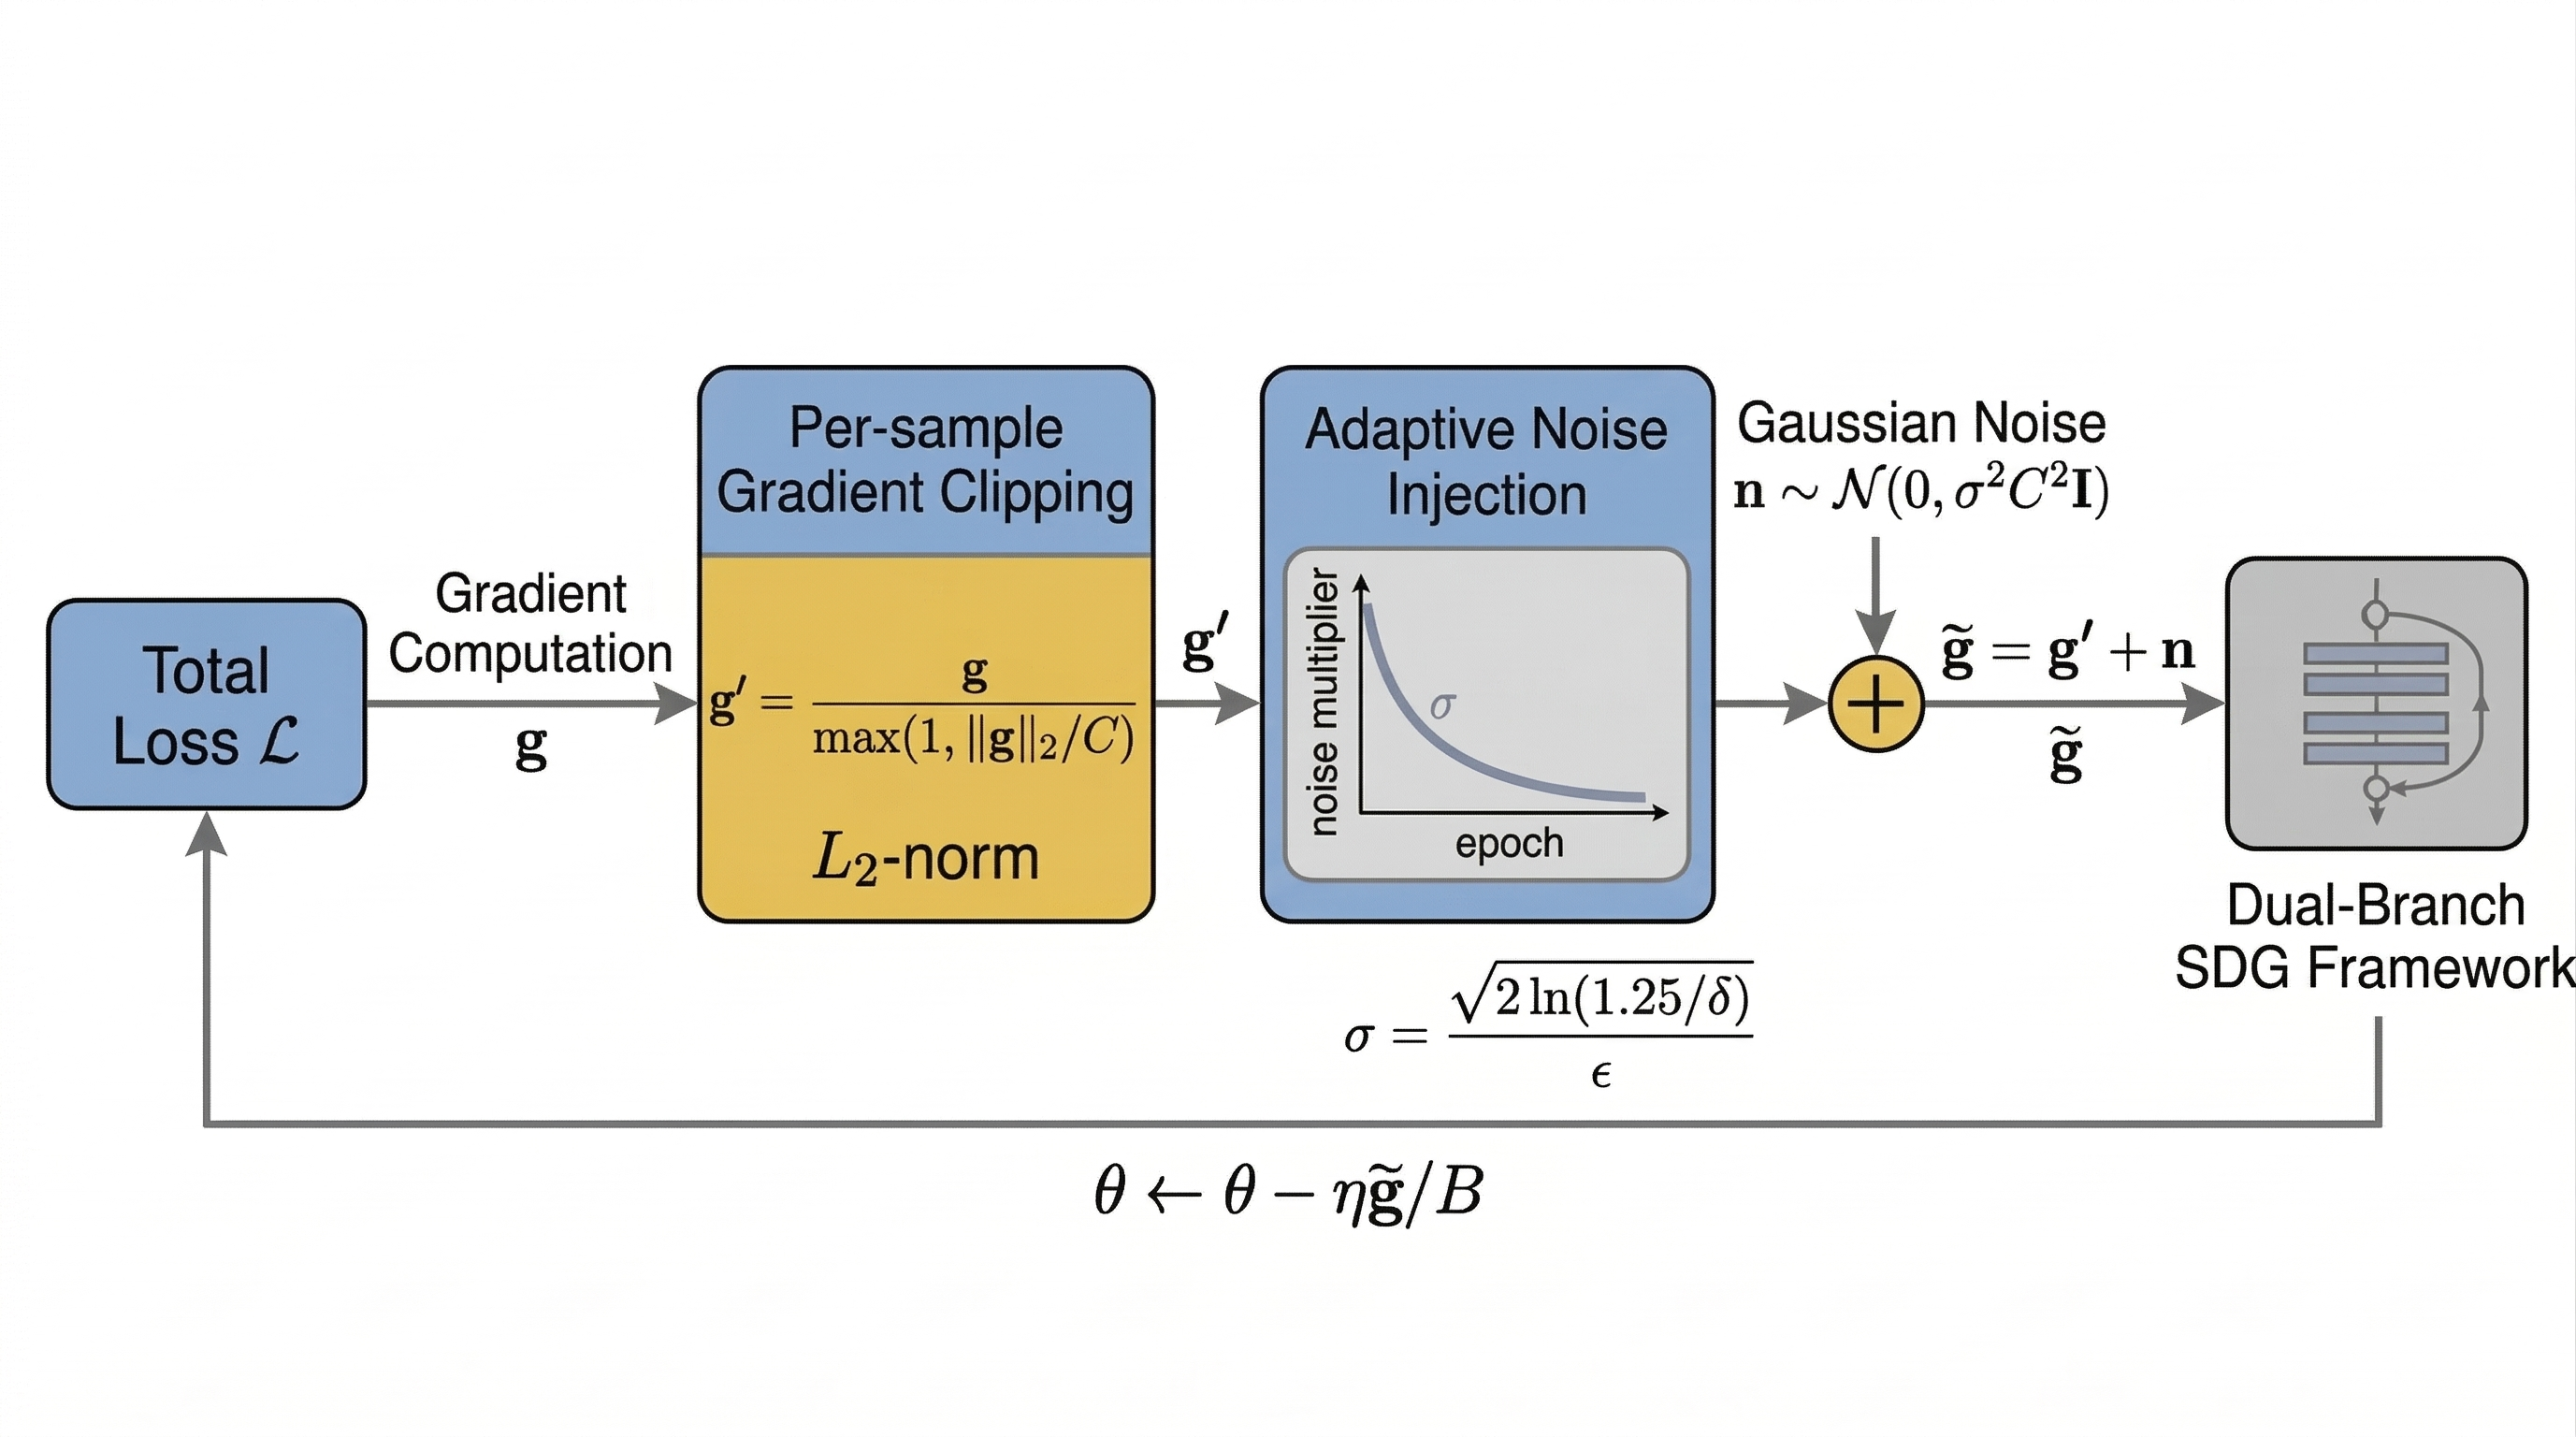
\includegraphics[width=0.82\textwidth]{./images/media/image3_v2.png}
\caption{自适应高斯差分隐私在单域泛化框架中的集成方式。训练过程中，每步更新均先对样本梯度进行裁剪，再注入高斯噪声并完成参数更新；与固定噪声差分隐私不同，本文采用随训练阶段自适应调整并逐步衰减的噪声乘数，从而在训练前期提供较强隐私保护，在训练后期减小噪声对模型收敛的干扰，进而取得隐私-性能平衡。 Integration of Adaptive Gaussian Differential Privacy into the single domain generalization framework. During training, each update first clips per-sample gradients, then injects Gaussian noise and updates the parameters. Unlike fixed-noise differential privacy, this study adopts a noise multiplier that is adaptively adjusted and gradually decayed with the training stage, providing stronger privacy preservation early in training while reducing noise interference with model convergence in later stages, thereby achieving a privacy-performance trade-off.}
\label{fig:privacy-framework}
\end{figure}

高斯差分隐私（GDP）通过在每步梯度更新时加入独立同分布的高斯噪声实现\((\epsilon, \delta)\)-差分隐私。对于相邻数据集\(D\)和\(D'\)（仅相差一个样本），若随机算法\(M\)对任意输出集合\(S\)满足：

Gaussian differential privacy (GDP) provides \((\epsilon, \delta)\)-differential privacy by adding independent and identically distributed Gaussian noise at each gradient update. For adjacent datasets \(D\) and \(D'\), which differ by only one sample, a randomized algorithm \(M\) satisfies \((\epsilon, \delta)\)-DP if, for any output set \(S\), it satisfies:

\[\Pr\lbrack M(D) \in S\rbrack \leq e^{\epsilon}\Pr\lbrack M(D') \in S\rbrack + \delta,
\]

则称\(M\)满足\((\epsilon, \delta)\)-DP，其中\(\epsilon\)衡量隐私保护程度，\(\delta\)为松弛项，通常设为\(10^{-5}\)。在DP-SGD框架下，每次迭代对每个样本梯度\(g\)先进行L2范数裁剪：

where \(\epsilon\) measures the degree of privacy preservation, and \(\delta\) is the relaxation parameter, usually set to \(10^{-5}\). Under the DP-SGD framework, the per-sample gradient \(g\) is first clipped by its L2 norm at each iteration:

\[g' = g/max(1, \parallel g \parallel_{2}/C),
\]

然后加入高斯噪声\(n \sim \mathcal{N}(0,\sigma^{2}C^{2}I)\)，其中\(\sigma\)为噪声乘数，用于控制噪声强度，通常与隐私预算\(\epsilon\)和松弛项\(\delta\)相关，可写为：

Gaussian noise \(n \sim \mathcal{N}(0,\sigma^{2}C^{2}I)\) is then added, where \(\sigma\) is the noise multiplier controlling noise intensity. It is usually related to the privacy budget \(\epsilon\) and relaxation parameter \(\delta\), and can be written as:

\[\sigma = \sqrt{2\ln(1.25/\delta)}/\epsilon.
\]

噪声梯度\(\widetilde{g} = g' + n\)，更新\(\theta \leftarrow \theta - \eta\widetilde{g}/B\)，其中\(B\)是批次大小。该过程通过注入噪声模糊梯度，防止逆向攻击恢复原始图像或标签。有关隐私保护机制及其安全性的详细证明，请参阅Dwork C et al.\hyperref[_Ref214903493]{{[}45{]}}的工作。

The noisy gradient is \(\widetilde{g} = g' + n\), and the parameters are updated as \(\theta \leftarrow \theta - \eta\widetilde{g}/B\), where \(B\) is the batch size. This process obscures gradients through noise injection and prevents inversion attacks from recovering original images or labels. Detailed theoretical guarantees for privacy-preserving mechanisms are provided by Dwork C et al.\hyperref[_Ref214903493]{{[}45{]}}.

然而，传统GDP在整个训练过程中使用固定\(\sigma\)，导致训练后期仍注入大量噪声，容易影响模型收敛和最终性能。为此，我们采用自适应高斯差分隐私优化器，在训练初期使用较大噪声乘数以提供较强保护，随后根据预设噪声衰减速率逐步降低噪声强度，以减小后期对模型收敛的影响。训练过程中，本文根据每轮噪声乘数、噪声衰减速率和采样过程累计隐私预算，并记录不同训练轮次下的\(\epsilon\)消耗与模型性能变化，用于分析隐私预算增长过程中的性能演化。最终实验验证，在中等隐私预算下，所提方法能够缓解噪声注入带来的性能下降，在隐私保护与模型性能之间取得较好的平衡。

However, conventional GDP uses a fixed \(\sigma\) throughout training, so substantial noise is still injected in later training stages, which can affect model convergence and final performance. Therefore, we adopt an Adaptive Gaussian Differential Privacy optimizer. A larger noise multiplier is used early in training to provide stronger protection, and the noise intensity is then gradually reduced according to a predefined noise decay rate to limit the impact of noise on model convergence in later stages. During training, this study accumulates the privacy budget according to the noise multiplier, noise decay rate, and sampling process of each epoch, and records \(\epsilon\) consumption and model performance at different training epochs to analyze performance evolution as the privacy budget increases. The final experiments show that, under a moderate privacy budget, the proposed method can alleviate the performance degradation caused by noise injection and achieve a good balance between privacy preservation and model performance.
